\documentclass{article}[12pt]
\usepackage{verbatim}
\usepackage{graphicx}

\title{CS246 Assignment 0}
\author{Nissan Pow}

\begin{document}
\maketitle

\section*{Part 1: C++ Basics}

1. In the declaration statement {\em int* a = 3}, the {\em *} indicates that {\em a} is a pointer to an int. In the assignment {\em b = *a}, the {\em *} is the dereference operator, and returns the object pointed to by the pointer (ie the value of the pointer). \\

In the declaration statement {\em int\& a = 3}, the {\em \&} indicates that {\em a} is a reference to another object of type int. In the assignment statement {\em b = \&a}, the {\em \&} returns the address of {\em a}.\\

2. A ``statically declared variable'' is created on the stack. \\

3. Code to dynamically declare a 2-D array and initialize it to form a 10x10 identity matrix.

\verbatiminput{array.C}

4. The code will output: {\em ``All Conditions Fail''}.

if {\em ((int)a == b)} is comparing the address of {\em new int(100)} with 100, and the address is very unlikely to be 100 so this condition will fail. \\

if {\em ((int)\&b == c)} is comparing the address of {\em b} with 100, so it will fail with the same reason as above. \\

if {\em ((int)a != b \&\& (int)\&b != c)} will be true, since both of the above are false. \\

\section*{Part 2: Reproduce a UML Diagram}

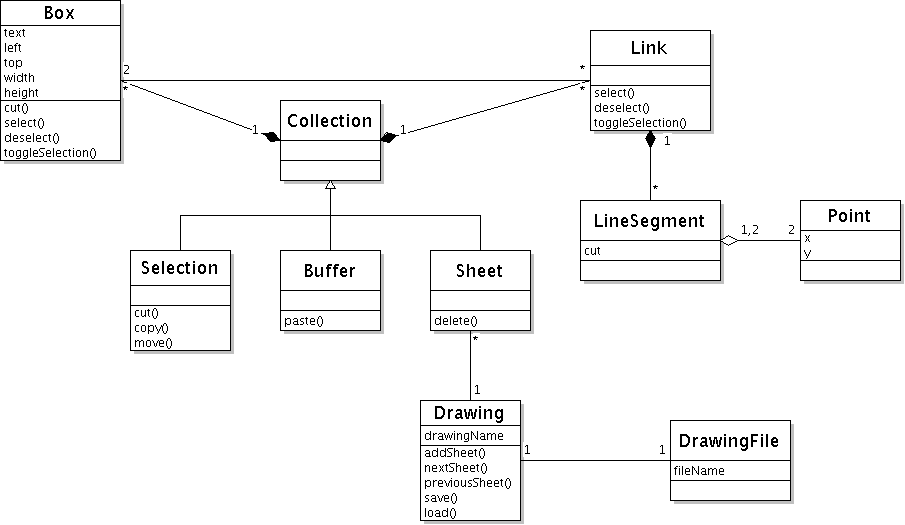
\includegraphics[scale=0.45]{cs246_a0.png}

\end{document}

